\documentclass[xetex,mathserif,serif]{beamer}
\usepackage[export]{adjustbox}


%\usetheme{Darmstadt}
%\usecolortheme{beetle}
\usetheme{Madrid}
\useoutertheme{miniframes} % Alternatively: miniframes, infolines, split
\useinnertheme{circles}

\definecolor{UBCblue}{rgb}{0.29412, 0.2745, 0.53334} % UBC Blue (primary)

\usecolortheme[named=UBCblue]{structure}
%\usecolortheme[named=Mahogany]{structure} % Sample dvipsnames color

\usepackage{graphicx}
\makeatletter
\providecommand{\bigsqcap}{%
  \mathop{%
    \mathpalette\@updown\bigsqcup
  }%
}
\newcommand*{\@updown}[2]{%
  \rotatebox[origin=c]{180}{$\m@th#1#2$}%
}
\makeatother


\title % (optional, only for long titles)
{Apstraktna interpretacija u modernim kompajlerima}
\subtitle{Seminarski rad u okviru kursa Metodologija stručnog i naučnog rada}
\author[Demonja, Maksimović, Crnobrnja] % (optional, for multiple authors)
{O.~Demonja, S.~Maksimović i M.~Crnobrnja}
\institute% (optional)
{
  Matematički fakultet\\
  Univerzitet u beogradu
}
\date % (optional)



\begin{document}
  \frame{\titlepage}
  \begin{frame}
    \frametitle{Formalizacija}
	    \framesubtitle{Skupovi konkretnih i apstraktnih stanja}
		\begin{center}
			\begin{itemize}
				\item $v \in V$ skup konkretnih stanja; \pause $v_{1} \rightsquigarrow v_{2}$ \emph{relacija} prelaska \pause
				%\item $... \rightsquigarrow v_{n} \rightsquigarrow v_{n}$ zaustavljanja programa
				\item $l \in L$ prostor svojstava; \pause $l_{1} \rightarrow l_{2}$ \emph{funkcija} prelaska \pause
				\item $\sqsubseteq \; \; \subset \; L \times L$ relacija poretka nad $L$ \pause
%				\begin{itemize}
%					\item $a \sqsubseteq a$ refleksivnost
%					\item $a \sqsubseteq b \wedge b \sqsubseteq a \implies a = b$ antisimetričnost
%					\item $a \sqsubseteq b \wedge b \sqsubseteq c \implies a \sqsubseteq c$ tranzitivnost
%				\end{itemize}
				\item $( L, \bigsqcup, \bigsqcap)$ potpuna mreža \pause
				\begin{itemize}
					\item $\forall l_0 \in L^{\prime} \; \; l_0 \sqsubseteq \bigsqcup_{l \in L^{\prime}} l$ %\pause
					\item $\forall l_0 (\forall l \in L^{\prime} \; l \sqsubseteq	l_0) \implies \bigsqcup_{l \in L^{\prime}} l \sqsubseteq l_0 $ \pause
					\item analogno za $\bigsqcap_{l \in L^{\prime}} l$ ... \pause
				\end{itemize}
				\item $\rho \subset V \times L$ relacija ispravnosti
				\begin{figure}
					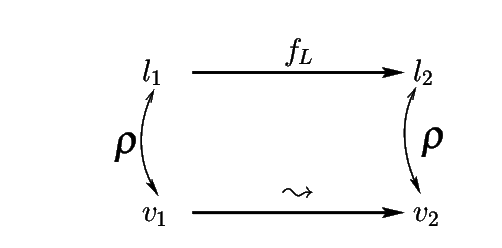
\includegraphics[scale=0.3,left]{Rho.png}
				\end{figure}
			\end{itemize}
		\end{center}
  \end{frame}
  \begin{frame}
    \frametitle{Formalizacija}
    \framesubtitle{Fiksne tačke}
	\begin{center}
		\begin{itemize}
			%\item $l \sqsubseteq \gamma(\alpha(l))$ \pause
			\item $x = f_{L}(x)$, \pause čine potpunu mrežu ukoliko je $f_{L}$ monotona.\pause
			\item $f^{0}_{L}(\bot) = \bot, \quad f^{n+1}_{L}(\bot) = f_{L}(f^{n}_{L}(\bot))$ \pause
			\item $\bigsqcup \{ \: f^{n}_{L}(\bot)\: \}_{n \in \mathbb{N}}$ je najmanja fiksna tačka \pause
			\begin{itemize}
				\item nepraktično za izračunati			\pause
			\end{itemize}
			\item uvodimo prostor $M$ i \emph{Galoaovu vezu}  $\langle L, \alpha, \gamma, M \rangle$
		\end{itemize}
		\begin{figure}
			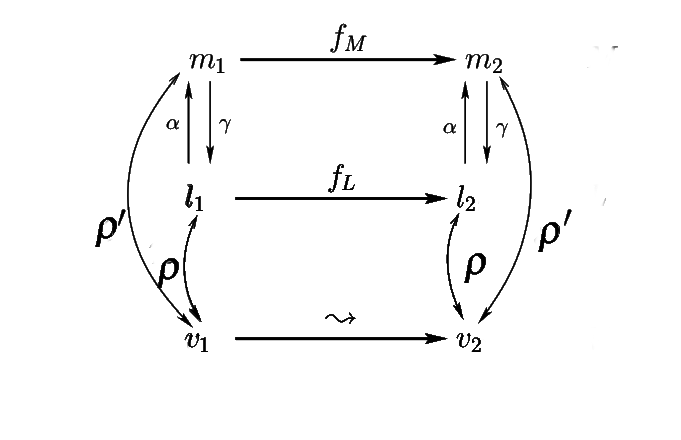
\includegraphics[scale=0.3,left]{Rho_prime.png}
		\end{figure}
		\end{center}
  \end{frame}
  \begin{frame}
    \frametitle{Formalizacija}
    \framesubtitle{Operator proširenja}
    \begin{center}
    	\begin{itemize}
    		\item $\nabla : L \times L \rightarrow L$ ubrzava konvergenciju \pause
    		\item $\forall x,\! y \; x \sqsubseteq x \nabla y, y \sqsubseteq x \nabla y$ \pause
    		\item $x^{\prime}_{0} = y_{0}, \; x^{\prime}_{n} = x^{\prime}_{n-1} \nabla y_{n}$ tada $(x^{\prime}_{n})_{n}$ konvergira u konačnom broju koraka \pause
    	\end{itemize}
    	$$
			f^{n}_{\nabla} = 
			\begin{cases}
			\bot,            								  
				& 	\text{za} \quad n = 0 \\
			f^{n-1}_{\nabla} 							      
				& \text{za} \quad n > 0 \quad \text{i} \quad f_{L}(f^{n-1}_{\nabla}) \sqsubseteq f^{n-1}_{\nabla} \\
			f^{n-1}_{\nabla} \nabla f_{L}(f^{n-1}_{\nabla})  
				& \text{inače}
			\end{cases}
		$$
	\end{center}
  \end{frame}
  \begin{frame}
    \frametitle{Formalizacija}
    \begin{figure}
		\begin{center}
		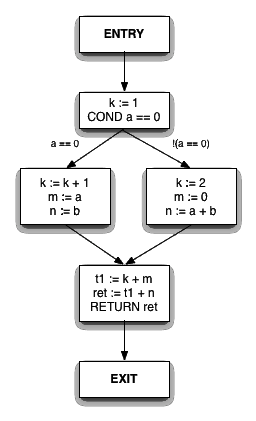
\includegraphics[scale=0.5]{Treehydra-cfg.png}
		\end{center}
	\end{figure}
  \end{frame}
  
% etc
\end{document}